\documentclass[11pt]{article}

\usepackage[a4paper,margin=1in]{geometry}
\usepackage[T1]{fontenc}
\usepackage[utf8]{inputenc}
\usepackage{lmodern}
\usepackage{amsmath,amssymb,amsthm,mathtools}
\usepackage{microtype}
\usepackage{xcolor}
\usepackage{hyperref}
\usepackage{enumitem}
\usepackage{booktabs}
\usepackage{array}
\usepackage{tikz}
\usepackage[most]{tcolorbox}
\usepackage{fancyhdr}
\usepackage{titlesec}
\usepackage{setspace}

\usetikzlibrary{arrows.meta,positioning,calc,fit,shapes.geometric}

\hypersetup{
  colorlinks=true,
  linkcolor=blue!50!black,
  urlcolor=blue!50!black,
  pdftitle={Coding Theory: Introduction - Lecture Notes},
  pdfauthor={OpenAI}
}

\definecolor{ctdark}{HTML}{0A3A78}
\definecolor{ctteal}{HTML}{0D7C7C}
\definecolor{ctlight}{HTML}{EAF4F8}
\definecolor{ctgray}{HTML}{F5F7FA}

\titleformat{\section}{\Large\bfseries\color{ctdark}}{\thesection}{0.6em}{}
\titleformat{\subsection}{\large\bfseries\color{ctteal}}{\thesubsection}{0.6em}{}

\setlength{\parindent}{0pt}
\setlength{\parskip}{0.7em}
\setstretch{1.08}

\pagestyle{fancy}
\fancyhf{}
\lhead{Coding Theory: Introduction}
\rhead{\thepage}
\renewcommand{\headrulewidth}{0.4pt}
\setlength{\headheight}{14pt}

\newtcolorbox{definitionbox}[1]{
  colback=ctlight,
  colframe=ctdark,
  boxrule=0.8pt,
  arc=2mm,
  left=2mm,right=2mm,top=1.5mm,bottom=1.5mm,
  title=\textbf{#1}
}

\newtcolorbox{summarybox}[1]{
  colback=ctgray,
  colframe=ctteal,
  boxrule=0.8pt,
  arc=2mm,
  left=2mm,right=2mm,top=1.5mm,bottom=1.5mm,
  title=\textbf{#1}
}

\newcommand{\DataNode}[2]{%
  \node[draw, rounded corners=1.5pt, minimum width=1.55cm, minimum height=0.8cm, fill=white] (#1) {#2};
}

\newcommand{\CloudNode}[2]{%
  \node[draw, ellipse, align=center, minimum width=2.7cm, minimum height=1.25cm, fill=white] (#1) {#2};
}

\newcommand{\HeaderTriplet}{%
  \node[font=\small\bfseries\color{cyan!55!black}] at (0,1.25) {Transmitter};
  \node[font=\small\bfseries\color{blue!60!black}] at (4.0,1.25) {Channel};
  \node[font=\small\bfseries\color{ctdark}] at (8.0,1.25) {Receiver};
  \draw[line width=1.2pt, cyan!55!black] (-0.9,1.0)--(0.9,1.0);
  \draw[line width=1.2pt, blue!60!black] (3.05,1.0)--(4.95,1.0);
  \draw[line width=1.2pt, ctdark] (7.0,1.0)--(9.0,1.0);
}


\begin{document}
\pagenumbering{roman}

\begin{titlepage}
\centering
\vspace*{2.2cm}

{\Huge\bfseries\color{ctdark} Coding Theory: Introduction\par}
\vspace{0.5cm}
{\Large Lecture Note Version in LaTeX\par}
\vspace{1.2cm}

\begin{tcolorbox}[colback=ctlight,colframe=ctdark,width=0.88\textwidth,arc=2mm,boxrule=0.8pt]
These notes reorganize an introductory slide deck into a self-contained lecture note.
The goal is not only to transcribe the slides, but also to make the ideas readable as a
continuous mathematical document.
\end{tcolorbox}

\vfill

\begin{tabular}{>{\bfseries}p{0.25\textwidth}p{0.55\textwidth}}
Topic & Introductory coding theory \\
Focus & Reliability of transmission and storage \\
Main examples & Erasures, errors, discrete/continuous channels, storage, BEC \\
Document type & Clean article-style notes with TikZ diagrams
\end{tabular}

\vfill

{\large \today\par}
\end{titlepage}
\pagenumbering{arabic}

\tableofcontents
\newpage

\section{What is Coding Theory?}

\begin{definitionbox}{Basic idea}
Coding theory studies how to design mechanisms that allow us to recover or protect data
when the data is disturbed during transmission or storage.
\end{definitionbox}

At the most basic level, the problem is simple to state:
\[
\text{original data} \longrightarrow \text{perturbance or noise} \longrightarrow \text{corrupted data}.
\]
The mathematical goal is to infer the original information from what is received.

\begin{summarybox}{Core goal}
Given corrupted data, recover the intended data as reliably as possible.
\end{summarybox}

\begin{center}
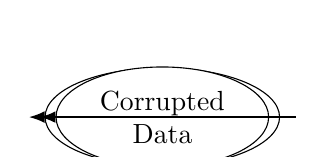
\begin{tikzpicture}[scale=1]
  \CloudNode{d}{Data}
  \CloudNode{n}{Perturbance}
  \CloudNode{c}{Corrupted\\Data}
  \draw[-{Latex[length=2mm,width=1.5mm]}, thick] ($(d.east)+(0.2,0)$) -- ($(n.west)+(-0.2,0)$);
  \draw[-{Latex[length=2mm,width=1.5mm]}, thick] ($(n.east)+(0.2,0)$) -- ($(c.west)+(-0.2,0)$);
\end{tikzpicture}
\end{center}

This introductory picture already contains the main philosophy of the subject: we do not
usually control the channel or storage medium perfectly, so instead we design redundancy,
structure, and decoding rules that make recovery possible.

\section{Communication and Storage Models}

Coding theory is usually explained through a channel model. A sender transmits data,
a channel perturbs it, and a receiver observes an altered version.

\subsection{Communication channel model}

\begin{center}
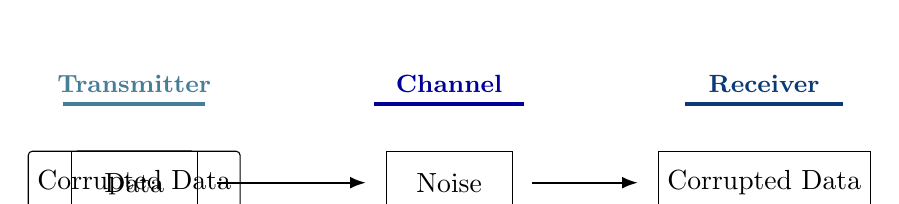
\begin{tikzpicture}[x=1cm,y=1cm]
  \HeaderTriplet
  \DataNode{x}{Data}
  \DataNode{z}{Noise}
  \DataNode{y}{Corrupted Data}
  \node at (0,-0.2) {};
  \path (0,0) node (x) [draw, minimum width=1.6cm, minimum height=0.8cm] {Data};
  \path (4,0) node (z) [draw, minimum width=1.6cm, minimum height=0.8cm] {Noise};
  \path (8,0) node (y) [draw, minimum width=2.5cm, minimum height=0.8cm] {Corrupted Data};
  \draw[-{Latex[length=2mm,width=1.5mm]}, thick] ($(x.east)+(0.25,0)$) -- ($(z.west)+(-0.25,0)$);
  \draw[-{Latex[length=2mm,width=1.5mm]}, thick] ($(z.east)+(0.25,0)$) -- ($(y.west)+(-0.25,0)$);
\end{tikzpicture}
\end{center}

A communication system can be abstracted as
\[
\text{transmitter} \longrightarrow \text{channel} \longrightarrow \text{receiver}.
\]
The channel introduces uncertainty, commonly modeled as noise.

\subsection{Erasure channels}

An \emph{erasure} means that some positions are lost, but the receiver knows exactly
which positions are missing.

\[
(x_1,x_2,x_3,x_4,x_5) \longrightarrow \text{erasures} \longrightarrow (x_1,\ast,x_3,\ast,\ast).
\]

This is easier than arbitrary error correction, because the receiver is told where the
uncertainty occurs.

\begin{summarybox}{Erasures vs. errors}
In an erasure channel, the bad locations are visible. In an error channel, the bad
locations are typically invisible.
\end{summarybox}

\subsection{Channels with errors}

In an error channel, transmitted symbols may be changed:
\[
(x_1,x_2,x_3,x_4,x_5) \longrightarrow \text{errors} \longrightarrow (y_1,y_2,y_3,y_4,y_5).
\]
Usually we do \emph{not} know where or when the errors occurred. That is why error
correction is subtler than erasure correction.

\subsection{Discrete channels with errors}

For a discrete channel, the symbols belong to a finite alphabet $A$:
\[
(x_1,x_2,x_3,x_4,x_5) \in A^5, \qquad |A| < \infty.
\]
The received word also lies in $A^5$, but some coordinates may have changed.
This is the classical setting for block codes over finite alphabets.

\subsection{Continuous channels with errors}

In a continuous channel, transmitted vectors live in a continuous space such as
$\mathbb{R}^5$ or $\mathbb{C}^5$:
\[
(x_1,x_2,x_3,x_4,x_5) \in \mathbb{R}^5 \text{ or } \mathbb{C}^5.
\]
This model is closer to many physical communication systems, where signals are analog
or are represented by real/complex amplitudes.

\subsection{Multi-input multi-output channels}

A MIMO channel can be modeled by a matrix input and matrix output, for example
\[
X = \begin{bmatrix}x_{11} & x_{12} \\ x_{21} & x_{22}\end{bmatrix} \in \mathbb{C}^{2\times 2},
\qquad
Y = \begin{bmatrix}y_{11} & y_{12} \\ y_{21} & y_{22}\end{bmatrix} \in \mathbb{C}^{2\times 2}.
\]
This reflects settings where multiple antennas transmit and receive simultaneously.

\subsection{Storage systems}

Coding theory is not only about sending data through space. It also applies to storing
data over time:
\[
\text{write/put} \longrightarrow \text{storage medium} \longrightarrow \text{read/get}.
\]
Noise or faults in the storage medium can corrupt the retrieved information.

\begin{center}
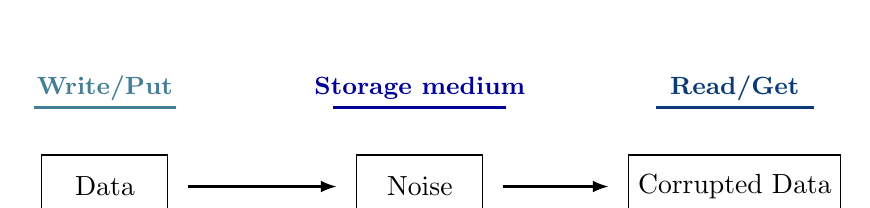
\begin{tikzpicture}[x=1cm,y=1cm]
  \node[font=\small\bfseries\color{cyan!55!black}] at (0,1.25) {Write/Put};
  \node[font=\small\bfseries\color{blue!60!black}] at (4.0,1.25) {Storage medium};
  \node[font=\small\bfseries\color{ctdark}] at (8.0,1.25) {Read/Get};
  \draw[line width=1.2pt, cyan!55!black] (-0.9,1.0)--(0.9,1.0);
  \draw[line width=1.2pt, blue!60!black] (2.9,1.0)--(5.1,1.0);
  \draw[line width=1.2pt, ctdark] (7.0,1.0)--(9.0,1.0);
  \path (0,0) node (x) [draw, minimum width=1.6cm, minimum height=0.8cm] {Data};
  \path (4,0) node (z) [draw, minimum width=1.6cm, minimum height=0.8cm] {Noise};
  \path (8,0) node (y) [draw, minimum width=2.5cm, minimum height=0.8cm] {Corrupted Data};
  \draw[-{Latex[length=2mm,width=1.5mm]}, thick] ($(x.east)+(0.25,0)$) -- ($(z.west)+(-0.25,0)$);
  \draw[-{Latex[length=2mm,width=1.5mm]}, thick] ($(z.east)+(0.25,0)$) -- ($(y.west)+(-0.25,0)$);
\end{tikzpicture}
\end{center}

The same erasure and error ideas appear here as well. For storage systems,
\emph{transmission/reception} is replaced by \emph{put/get} operations.

\section{Coding Theory as a Subject}

A compact description is:

\begin{definitionbox}{Working definition}
Coding theory is the study of the design of mechanisms that ensure reliability of data
transmission in the presence of perturbance. For storage systems, the same viewpoint
applies with write/read operations in place of transmit/receive operations.
\end{definitionbox}

In many introductory courses, the emphasis is placed on transmission through discrete
channels, because that setting already contains the central ideas of encoding, redundancy,
and decoding.

\section{Related Areas}

Coding theory sits naturally between several nearby disciplines.

\begin{center}
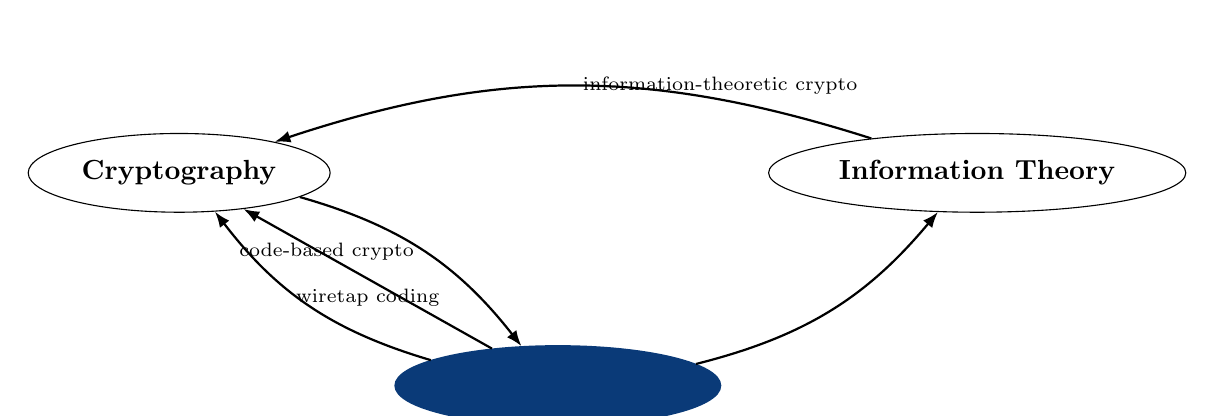
\begin{tikzpicture}[node distance=2.8cm]
  \node[draw, ellipse, minimum width=3.1cm, minimum height=1cm, fill=ctlight, thick, color=ctdark] (ct) {\textbf{Coding Theory}};
  \node[draw, ellipse, minimum width=3.0cm, minimum height=1cm, fill=white, above left=of ct] (cr) {\textbf{Cryptography}};
  \node[draw, ellipse, minimum width=3.5cm, minimum height=1cm, fill=white, above right=of ct] (it) {\textbf{Information Theory}};

  \draw[-{Latex[length=2mm,width=1.5mm]}, thick] (ct) to[bend left=18] node[midway, below] { } (cr);
  \draw[-{Latex[length=2mm,width=1.5mm]}, thick] (cr) to[bend left=18] node[midway, left, font=\scriptsize] {code-based crypto} (ct);
  \draw[-{Latex[length=2mm,width=1.5mm]}, thick] (ct) to[bend right=18] node[midway, below] { } (it);
  \draw[-{Latex[length=2mm,width=1.5mm]}, thick] (it) to[bend right=18] node[midway, right, font=\scriptsize] {information-theoretic crypto} (cr);
  \draw[-{Latex[length=2mm,width=1.5mm]}, thick] (ct) -- node[midway, below, font=\scriptsize] {wiretap coding} (cr);
\end{tikzpicture}
\end{center}

\begin{itemize}[leftmargin=2em]
  \item \textbf{Information theory} studies fundamental limits on communication, such as
  capacity, compression, and noise tolerance.
  \item \textbf{Cryptography} studies secrecy, authenticity, and adversarial security.
  \item \textbf{Coding theory} overlaps with both: for example, code-based cryptography and
  wiretap coding lie directly at these interfaces.
\end{itemize}

\section{Applications}

Coding theory appears in many settings:

\begin{itemize}[leftmargin=2em]
  \item coding for communications (wired and wireless),
  \item coding for storage (CDs, RAID systems, cloud storage),
  \item network coding,
  \item coding for memories,
  \item quantum coding,
  \item source coding and compression.
\end{itemize}

\begin{summarybox}{Why coding theory matters}
The subject is not a narrow niche. It is a common mathematical language for reliability
across communication, storage, networking, and even quantum information.
\end{summarybox}

\section{The Binary Erasure Channel}

One of the simplest and most important toy models is the \emph{binary erasure channel}
(BEC).

\subsection{Definition}

The BEC has:
\begin{itemize}[leftmargin=2em]
  \item input alphabet $\{0,1\}$,
  \item output alphabet $\{0,1,\ast\}$,
  \item erasure probability $P_e$.
\end{itemize}

If the input bit is $0$, then the output is:
\[
0 \xrightarrow{1-P_e} 0, \qquad 0 \xrightarrow{P_e} \ast.
\]
If the input bit is $1$, then the output is:
\[
1 \xrightarrow{1-P_e} 1, \qquad 1 \xrightarrow{P_e} \ast.
\]

\begin{center}
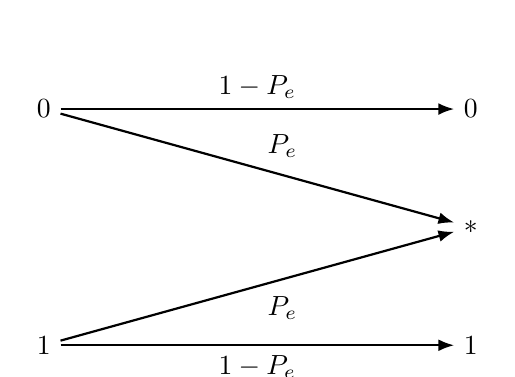
\begin{tikzpicture}[x=1cm,y=1cm]
  \node[left] (z0) at (0,1.5) {$0$};
  \node[left] (z1) at (0,-1.5) {$1$};
  \node[right] (o0) at (5,1.5) {$0$};
  \node[right] (o1) at (5,-1.5) {$1$};
  \node[right] (os) at (5,0) {$\ast$};

  \draw[-{Latex[length=2mm,width=1.5mm]}, thick] (z0) -- node[above] {$1-P_e$} (o0);
  \draw[-{Latex[length=2mm,width=1.5mm]}, thick] (z0) -- node[above right] {$P_e$} (os);
  \draw[-{Latex[length=2mm,width=1.5mm]}, thick] (z1) -- node[below right] {$P_e$} (os);
  \draw[-{Latex[length=2mm,width=1.5mm]}, thick] (z1) -- node[below] {$1-P_e$} (o1);
\end{tikzpicture}
\end{center}

\subsection{Interpretation}

The channel never flips $0$ into $1$ or $1$ into $0$. Instead, it either preserves the bit
or replaces it by an erasure symbol $\ast$. The benefit is that the receiver knows exactly
which coordinate was lost.

\subsection{Example of a transmitted word}

A binary input word such as
\[
(0,1,0,0,1) \in \{0,1\}^5
\]
may be received as
\[
(0,1,0,\ast,1).
\]
Only one coordinate was erased, and its position is visible.

\section{Conceptual Comparison of Channel Types}

\begin{center}
\renewcommand{\arraystretch}{1.35}
\begin{tabular}{>{\bfseries}p{0.24\textwidth}p{0.31\textwidth}p{0.31\textwidth}}
\toprule
Model & What happens? & What the receiver knows \\
\midrule
Erasure channel & Some symbols are replaced by $\ast$ or marked missing & The uncertain locations are known \\
Error channel & Some symbols are changed into other valid symbols & The uncertain locations are usually unknown \\
Discrete channel & Symbols come from a finite alphabet $A$ & Works with block codes over finite alphabets \\
Continuous channel & Symbols are real or complex valued & Noise is modeled in a continuous signal space \\
Storage model & Data degrades between write and read & Reliability is needed over time, not just distance \\
\bottomrule
\end{tabular}
\end{center}

\section{Why Redundancy Is Necessary}

Suppose a sender transmits data with no redundancy at all. Then any erased or corrupted
symbol may destroy information permanently. Coding theory answers this by replacing the
original message with a longer, more structured codeword.

Typical design principles include:
\begin{itemize}[leftmargin=2em]
  \item adding redundant symbols,
  \item choosing codewords with enough separation,
  \item designing efficient decoding rules,
  \item exploiting special channel knowledge (for example, erasure locations).
\end{itemize}

This introductory lecture does not yet build specific codes, but it sets up the language
used later when one studies Hamming distance, linear codes, parity checks, generator
matrices, syndrome decoding, channel capacity, and more advanced constructions.

\section{Short Summary}

\begin{summarybox}{Main takeaways}
\begin{enumerate}[leftmargin=2em]
  \item Coding theory studies reliable communication and storage in the presence of noise.
  \item The basic distinction is between \emph{erasures} and \emph{errors}.
  \item Models may be discrete, continuous, matrix-valued, or storage-based.
  \item The subject is closely related to information theory and cryptography.
  \item The binary erasure channel is a fundamental first example.
\end{enumerate}
\end{summarybox}

\section*{Possible next topics}
\addcontentsline{toc}{section}{Possible next topics}

If you continue these notes into a full course, natural next sections would be:
\begin{itemize}[leftmargin=2em]
  \item Hamming distance and nearest-neighbor decoding,
  \item block codes and linear codes,
  \item parity-check and generator matrices,
  \item erasure correction versus error correction,
  \item repetition codes, parity codes, and Hamming codes,
  \item channel capacity and Shannon's viewpoint.
\end{itemize}

\end{document}
